\newpage
\subsection{Exemplos de ferramentas}
\label{exemplosferramentasdsl}

\citeonline{fowler2005language}, apresenta em seu texto, a \textit{Intentional Software} como a precursora das ferramentas de criação de linguagens, foi desenvolvida por \textit{Charles Simonyi} no setor de pesquisa \textit{Microsoft Research}. 

Essa ferramenta permite a criação e edição de código de domínio, o qual é criado por meio da definição de um esquema de domínio pelo \textit{Domain Expert} com apoio dos desenvolvedores, para então ser construído um gerador de código que resulta na aplicação final \cite{simonyi2006intentional}. 

A ferramenta utiliza uma representação de domínio em formato de árvore de intenções, que é apresentada ao usuário em diferentes formas de visualização e edição, a Figura \ref{fig:intentional} mostra a árvore de intenção para uma instrução matemática simples.

\begin{figure}[h!]
\centering

\caption{\textmd{Árvore de intenção no \textit{Intentional Software}}}
\label{fig:intentional}
\fcolorbox{gray}{white}{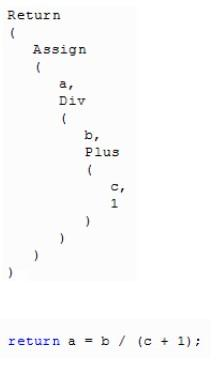
\includegraphics[width=0.4\textwidth]{chapters/fundamentacao/imagens/intentional.jpg}}

\par\medskip\textbf{Fonte:} \cite{simonyi2006intentional} \par\medskip
\end{figure}


Outra ferramenta de abordagem projecional é a \gls{MPS}, de código aberto sob a licença Apache 2.0 e é desenvolvida pela \textit{JetBrains}. Ela se baseia em definição de linguagens por meio de representação de texto estruturado, e possui uma série de recursos sofisticados de edição e ferramentas de navegação. 

Segundo \citeonline{dslengineering}, a \gls{MPS} suporta notações mistas (textuais, simbólicas, tabulares, gráficas) e uma ampla variedade de recursos de composição de idiomas. Ela define a linguagem por meio de \textit{Concepts} que são elementos para criação da sintaxe abstrata (Figura \ref{fig:mpsconceitos}), e esses conceitos são atrelados a um editor, o qual define as regras de projeção por meio de uma lista de células, que juntas definem a estrutura desejada para a sintaxe do conceito (Figura \ref{fig:mpseditor}).

\begin{figure}[h!]
\centering

\caption{\textmd{MPS definição de Conceitos}}
\label{fig:mpsconceitos}
\fcolorbox{gray}{white}{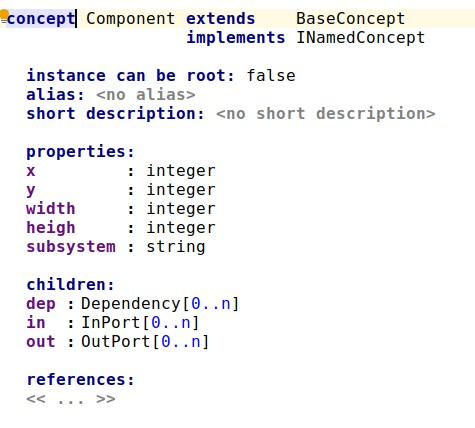
\includegraphics[width=\textwidth]{chapters/fundamentacao/imagens/mpsconceitos.jpg}}

\par\medskip\textbf{Fonte:} JetBrains (2018). \par\medskip
\end{figure}


\begin{figure}[ht!]
\centering

\caption{\textmd{MPS editor - sintaxe abstrata}}
\label{fig:mpseditor}
\fcolorbox{gray}{white}{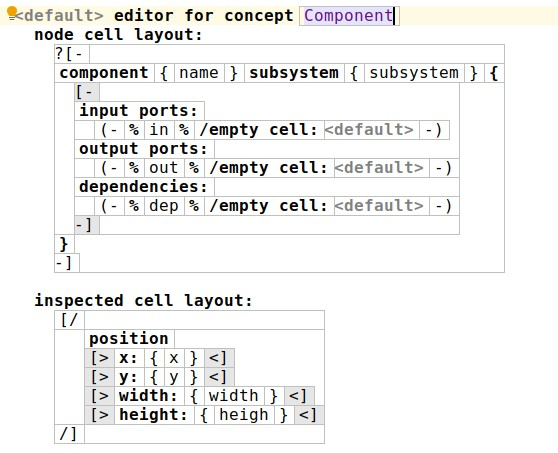
\includegraphics[width=0.98\textwidth]{chapters/fundamentacao/imagens/mpseditor.jpg}}

\par\medskip\textbf{Fonte:} JetBrains (2018). \par\medskip
\end{figure}


\newpage


Como alternativa às ferramentas projecionais, existem ferramentas que geram o \textit{parser} a partir da gramática, nesse caso, as regras da linguagem são expressadas em notação baseada em \gls{BNF}. As ferramentas Xtext e Spoofax são casos de ambientes nos quais é possível construir \gls{DSL}s por meio desse tipo de abordagem, a seguir são listados alguns exemplos nessas ferramentas.


\citeonline{eysholdt2010xtext}, descreve a ferramenta Xtext, como um \textit{framework} que permite o rápido desenvolvimento de ferramental de suporte às linguagens textuais, podendo atender desde linguagens menores como \gls{DSL}s, até linguagens completas \gls{GPL}s. Ela utiliza o core do \gls{EMF} para criar a \GLS{AST} a partir de uma especificação de gramática. 

Na Figura \ref{fig:xtextgramatica} é possível verificar a definição da gramática de uma linguagem específica para modelagem de entidades, de forma similar ao que existe em alguns \textit{frameworks} de programação, como Rails e Grails. O resultado é apresentado na Figura \ref{fig:xtextprograma}, na qual observa-se a utilização de recursos do Xtext no momento da codificação de um novo programa nessa linguagem.

\begin{figure}[ht!]
\centering

\caption{\textmd{Exemplo de definição de gramática Xtext}}
\label{fig:xtextgramatica}
\fcolorbox{gray}{white}{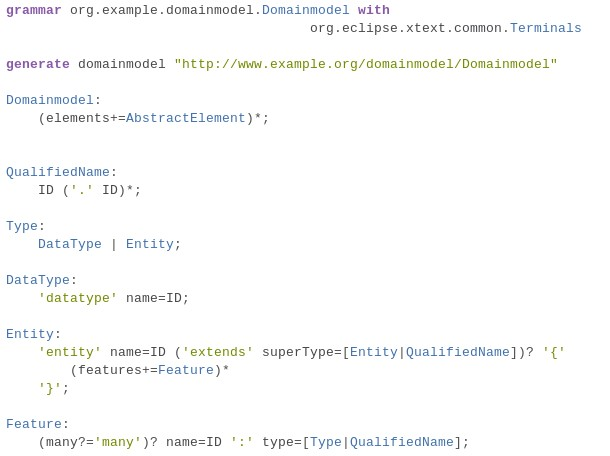
\includegraphics[width=0.9\textwidth]{chapters/fundamentacao/imagens/xtextgramatica.jpg}}

\par\medskip\textbf{Fonte:} \citeonline{xtextsite}. \par\medskip
\end{figure}


\begin{figure}[h!]
\centering

\caption{\textmd{Exemplo de uso da linguagem de entidades}}
\label{fig:xtextprograma}
\fcolorbox{gray}{white}{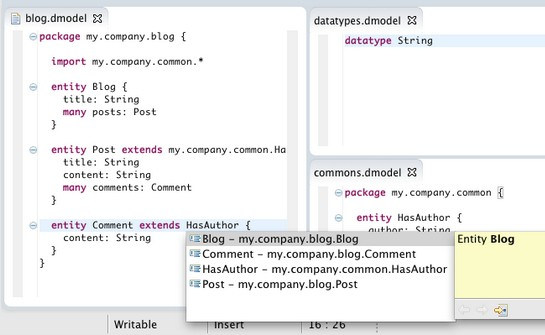
\includegraphics[width=0.9\textwidth]{chapters/fundamentacao/imagens/xtextprograma.jpg}}

\par\medskip\textbf{Fonte:} \citeonline{xtextsite}. \par\medskip
\end{figure}


\newpage
Por fim, a ferramenta \textit{Spoofax} utiliza o formato \gls{SDF} para descrição da sintaxe da linguagem, sendo um ambiente integrado de especificação de linguagens, com suporte e \textit{plugins} para a \gls{IDE} Eclipse. 

Um exemplo de definição de gramática em formato \gls{SDF} pode ser observado na Figura \ref{fig:spoofaxgramatica}. No canto esquerdo da imagem são definidas as regras da sintaxe, para uma linguagem de entidades similar a que foi utilizada no exemplo do Xtext. 

\begin{figure}[h!]
\centering

\caption{\textmd{Definição de gramática no Spoofax}}
\label{fig:spoofaxgramatica}
\fcolorbox{gray}{white}{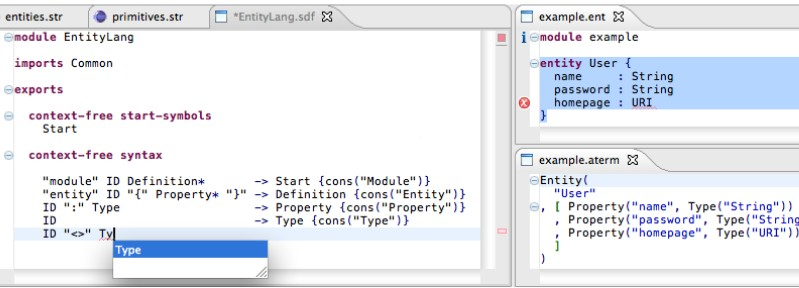
\includegraphics[width=0.9\textwidth]{chapters/fundamentacao/imagens/spoofaxgramatica.jpg}}

\par\medskip\textbf{Fonte:} \cite{kats2010spoofax} \par\medskip
\end{figure}



Segundo \citeonline{kats2010spoofax}, os seus editores permitem verificar e destacar erros por linha, validar tipos de dados da linguagem, resolução de referências, recursos de ajuda conforme contexto e até completar ou sugerir opções de código para o usuário da linguagem (Figura \ref{fig:spoofaxeditor}). 

\begin{figure}[h!]
\centering

\caption{\textmd{Recursos do editor Spoofax}}
\label{fig:spoofaxeditor}
\fcolorbox{gray}{white}{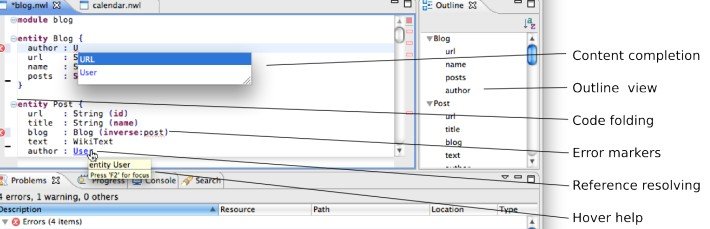
\includegraphics[width=\textwidth]{chapters/fundamentacao/imagens/spoofaxeditor.jpg}}

\par\medskip\textbf{Fonte:} \cite{kats2010spoofax} \par\medskip
\end{figure}


A fim de criar a linguagem de domínio proposta pelo presente trabalho, foi necessário definir entre uma dessas ferramentas. Na Seção \ref{justificativamps} é apresentada a justificativa da escolha do \gls{MPS} como ferramenta para implementação da linguagem de especificação de regras de classificação pelo sistema de cotas.